\chapter{Introduction}
\setcounter{page}{1}
\pagenumbering{arabic}


\shorthandoff{-} 
\section{Natural selection}
Bacteria exhibit genotypic and phenotypic variability even at the levels of genus.
This variability is continuously shaped by natural selection as the cells that are better adapted to the current conditions are more likely to survive and proliferate.
% the "drect experience" argument seems hard to make. I also experience the environment directly (perhaps my gametes do not?)
%%% BETTER OR DO YOU WANT ME TO CHANGE THE SENTENCE COMPLETELY? (ADDED limited ability to escape)
In the case of unicellular organisms the survival game is more stringent, because they face the changing conditions directly and have limited ability to escape.
Drought, nutrient poor environments, or high UV radiation are some of the most harsh environments bacteria can experience.
Nevertheless even in these we find viable cells which have evolved to survive for either short or long period of time.
% I don't quite understand "in the way how to overcome"
%%% BETTER?
Importantly, cells have evolved multiple ways how to overcome such conditions and thus variability in survival strategies in the same environment still occurs.
These differences could be driven by other selection forces acting simultaneously or could be a result of previous evolution in response to a similar environment.
Anyway, cells which don't manage to adapt to the new conditions are excluded by natural selection and die.
%%% SHOULD I FIND AND ADD SOME REFERENCES?


\section{Transcriptional networks}

\subsection{Cellular responses}
It is essential for a living cell to sense what is happening in the environment it is present at and react accordingly.
If reaction time, before death, is limited to seconds there is no time for change in transcription or translation level.
In that case the cell fate depends on the proteins it has already synthesised, and when none with an appropriate enzymatic activity is present, the cell dies.
Nice example of fast response to a signal is chemotaxis.
When a motile bacterium occurs in attractant (sugars, amino acids) or repellent (metabolites, some divalent cations) gradient, it swim towards or away from the higher concentration of it, respectively.
In order to react swiftly, the cell needs to have the flagella already expressed.

On the other hand the necessity to react in minutes or hours is enough to activate and silence appropriate genes.
Such transcriptional responses are adequate in slowly changing environments e.g. decrease in preferred carbon source concentration.
% could also put in SOS here. Might mention riboswitches if you want to talk about translation control?
%%% DO YOU WANT ME TO EXPAND THIS OR WAS IT JUST SUGGESTION, WHICH IS NOT NECESSARY TO DO?
When a non-preferred carbon source is present as well the cells are brought to decision whether to enter long-term stationary phase or begin to utilize the alternative carbon source.
In any case they have to alter their transcription accordingly.
To manage and orchestrate all possible responses to multiple signals cells evolved a network of extra- and intracellular signaling pathways.
As I focus on transcriptional responses the following text covers mostly these cases.

\subsubsection{Direct signalling pathways}
Direct signalling is a case when a signal molecule is imported through cell membrane into cytosol or is produced by the cell and subsequently interacts with gene regulatory protein.
This is often the case in the regulation of carbohydrate catabolism and amino acid biosynthesis genes \cite{charlier1992arginine, weickert1992isorepressor, pittard1996various, wheatley2013structural}.
Two simple models are described below.

Cells avoid wasteful production of proteins which are not used at all the time.
For instance, there is no sense in producing plenty of enzyme hydrolysing lactose (lacZ) if no lactose is present.
To achieve this, \tax{E. coli} expresses \tax{lac} repressor (LacI) \cite{hudson1990co}.
However, \tax{lac} operon transcription is desired if lactose is present in the media.
Here \tax{lac} operon inducers take a turn.
Allolactose - \tax{lac} operon inducer - is imported by lactose permease into the cell where it binds directly to the repressor LacI.
Lactose itself has to be modified to the allolactose by $\beta$-galactosidase (LacZ) at first \cite{jobe1972lac, wheatley2013structural}.
LacI binding to the promoter DNA is then released triggering \tax{lacZYA} expression (Fig. \ref{dir}\textcolor{red}{a}) together with binding of general regulatory protein CRP \cite{hudson1990co, clark2005molecular}.

\begin{figure}[ht]
  \centering
  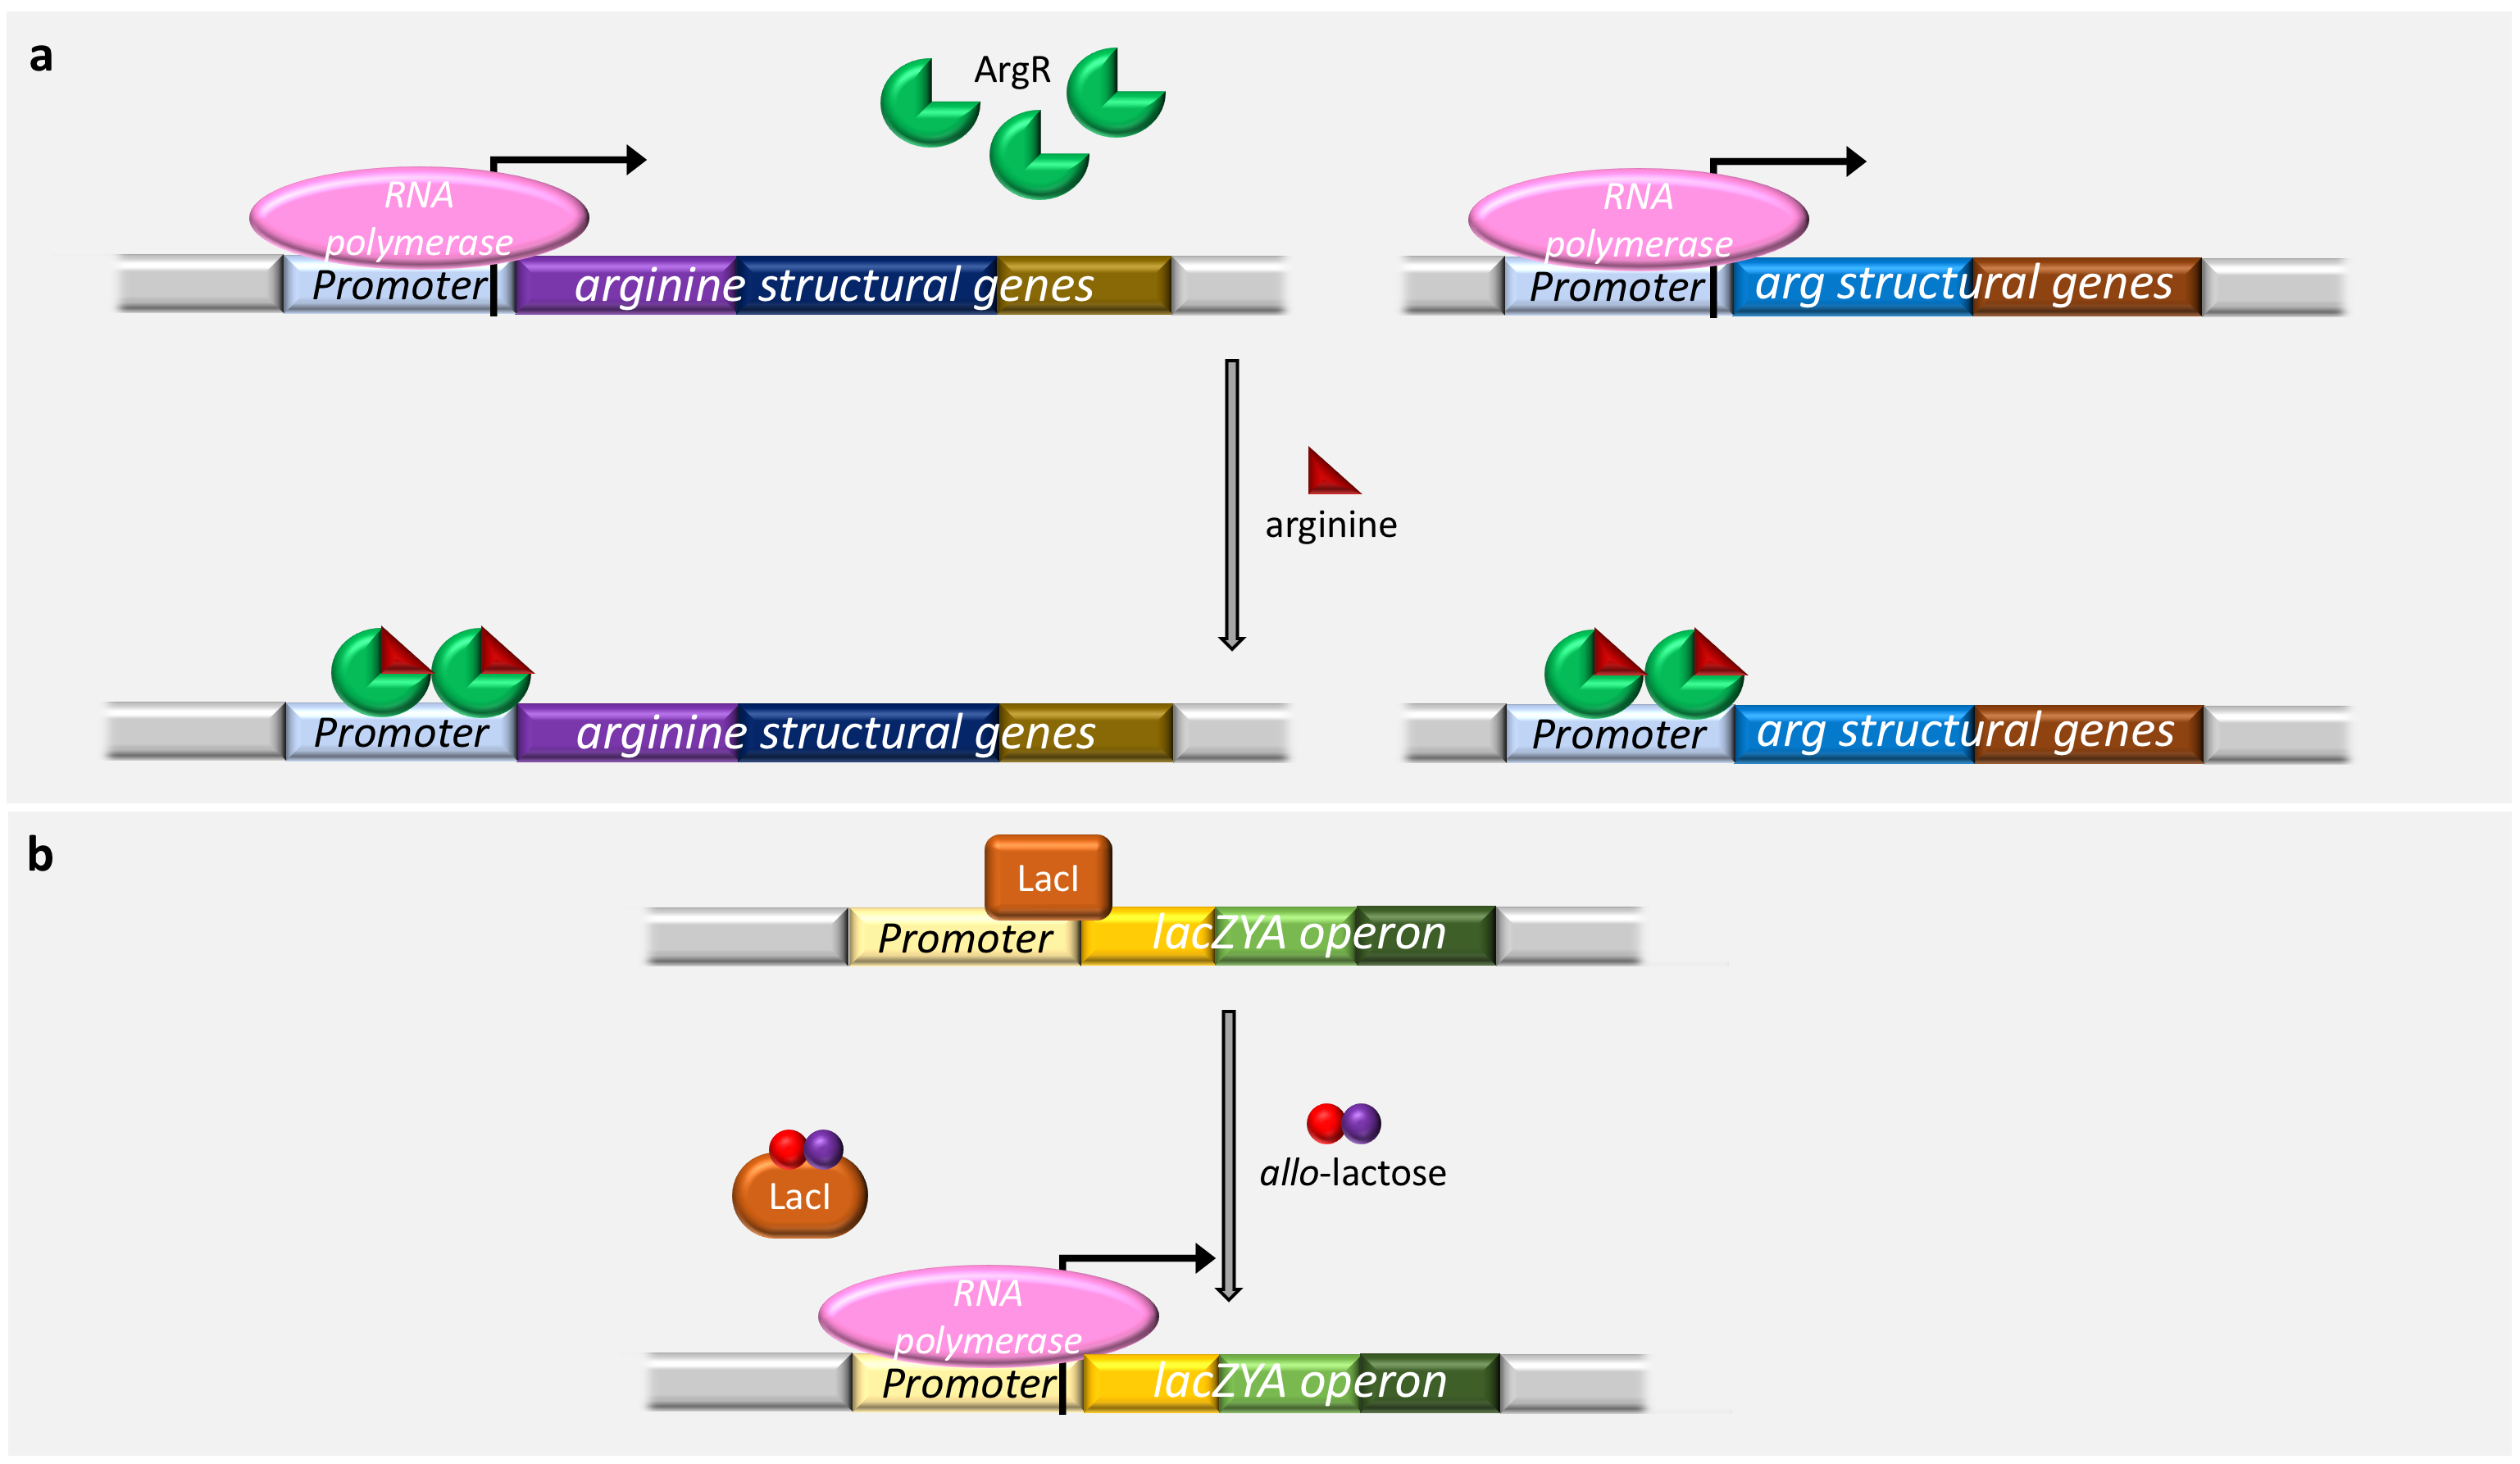
\includegraphics[scale=0.27]{text/Pictures/DirectSignaling.png}
	\caption{Scheme of direct signaling; \textbf{a} if \tax{lac} operon inducer (allolactose) is present it binds to LacI repressor and induces \tax{lac} operon transcription; \textbf{b} expression of arginine structural genes is co-repressed by arginine itself, because without it ArgR repressor cannot bind to DNA.}
	\label{dir}
\end{figure}

For other metabolic pathways things might work in a different way, however.
Arginine, for instance, acts as a co-repressor of its own biosynthesis (Fig. \ref{dir}\textcolor{red}{b}).
This means that when a bacterium does not have enough of this amino acid available for protein production the transcription of arginine genes is active \cite{charlier2004biosynthesis, caldara2006arginine}.
On the other hand, when arginine is abundant in the culture medium and thus in the cell, there is no need to make more of it.
The cell has ArgR repressor present in cytosol but ArgR itself cannot bind to DNA and inhibit transcription in the arginine absence \cite{clark2005molecular, caldara2006arginine}.
However when there is plenty of arginine in the cell it binds to ArgR and as a co-repressor inhibits expression of arginine structural genes binding to an appropriate promoter \cite{charlier1992arginine, charlier2004biosynthesis, clark2005molecular}.

\subsubsection{Indirect signalling pathways}
A classic example of indirect signalling is two-component system.
It consists of a transmembrane sensory kinase which is autophosphorylated at its histidine residue after receiving physical or chemical signal from the environment (Fig. \ref{two}\textcolor{red}{a}).
To be able to phosphorylate itself the kinase requires ATP or other phosphate donor.
Next, the phosphorylated kinase transfers the phosphate group to its partner regulatory protein enabling its activity, most often DNA-binding and transcriptional regulation \cite{lynch2012prioritization, gao2015temporal, cui2018novel}.
This protein receives the phosphate to its aspartate residue and might act as both gene repressor and/or activator.
Alternatively, the output of the two-component system can be a modification of biochemical activity of target proteins or RNAs instead or on the top of the change in gene expression \cite{shu2002antar, chambonnier2016hybrid}.

The described kinases and cognate regulatory proteins do not necessarily need to be separated units.
Proteins with histidine kinase domains connected to aspartate domains of DNA-binding proteins are known.
These hybrid systems are usually located in cell membrane with their sensory domains in periplasmic space (Fig. \ref{two}\textcolor{red}{b}) \cite{lynch2012prioritization, hirano2013regulon}.

\begin{figure}[h!]
  \centering
  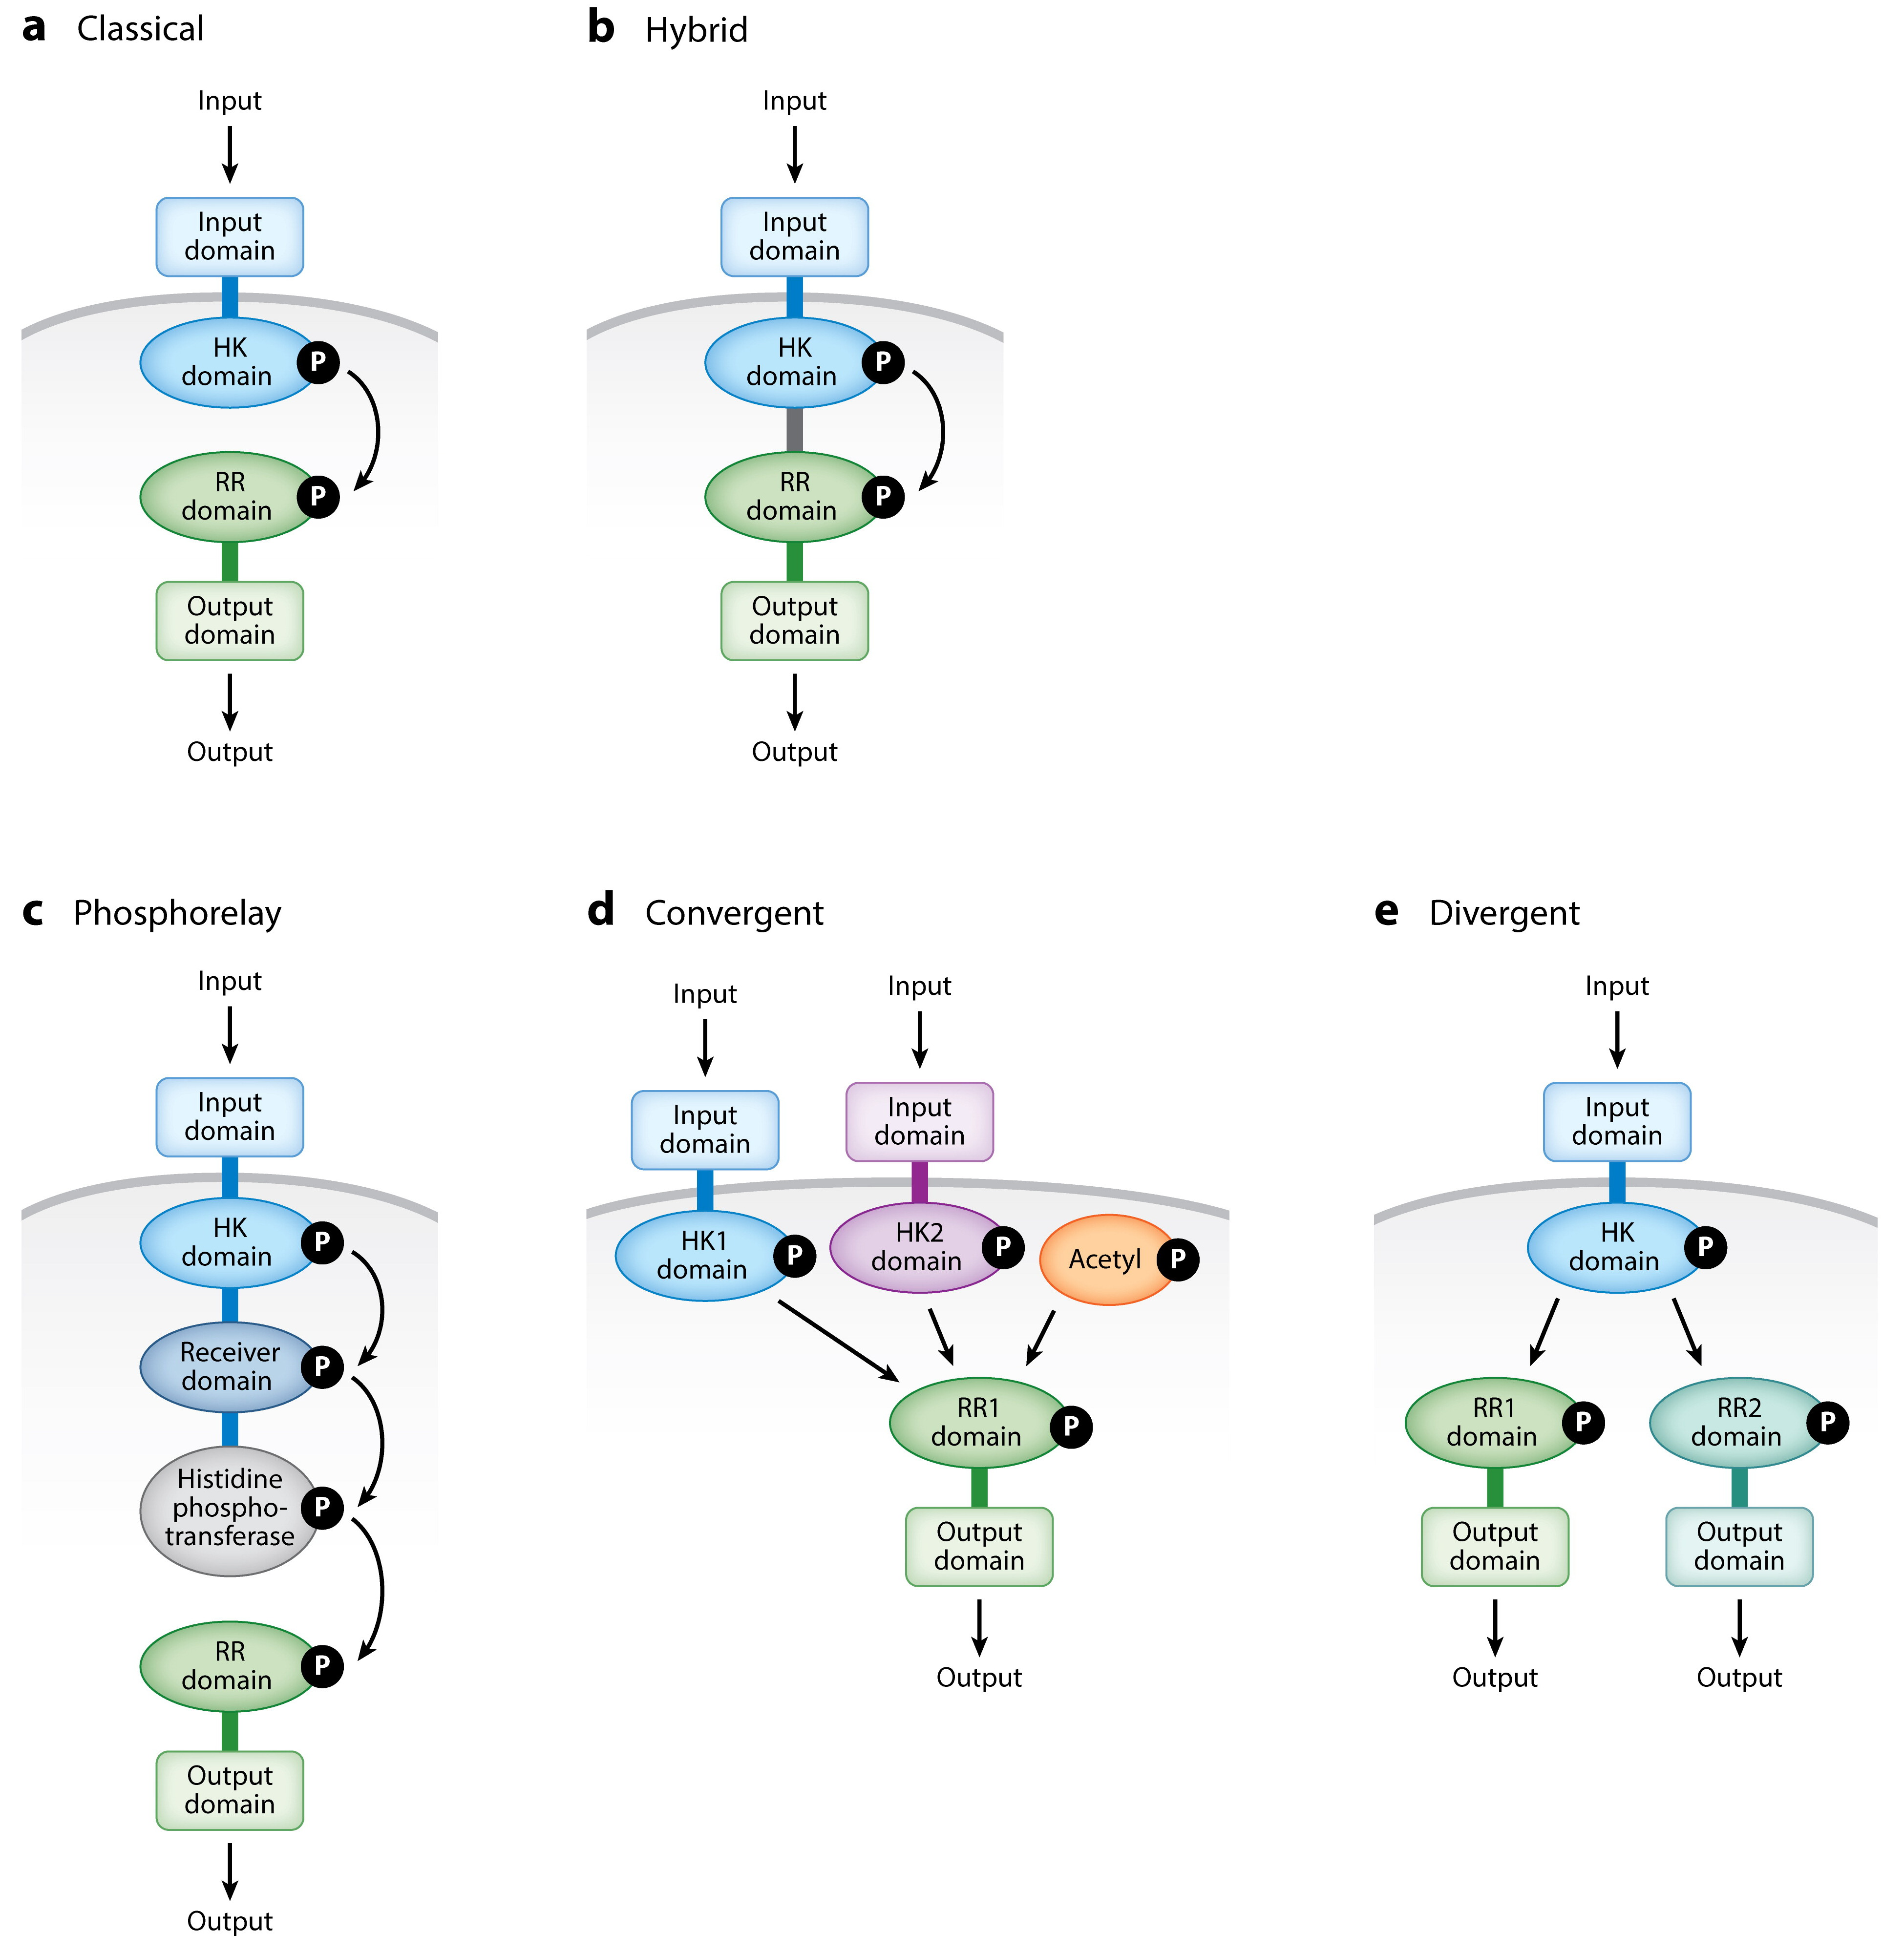
\includegraphics[scale=0.85]{text/Pictures/TwoComponent.jpeg}
	\caption{Two-component signaling pathways; \textbf{a} histidine kinase (HK) autophosphorylates in response to a signal and subsequently transfers the phosphate to a response regulator (RR) which generates output; \textbf{b} a hybrid system comprises both components (HK and RR) into a single protein; \textbf{c} in phosphorelay the phosphate is transferred multiple times before reaching its final RR; \textbf{d} some RR can be activated by several HK including metabolites such as acetyl phosphate; \textbf{e} one HK might phosphorylate multiple RR generating various outputs. (reproduced from \cite{groisman2016feedback})}
	\label{two}
\end{figure}

Another version of two-component system is phosphorelay (Fig. \ref{two}\textcolor{red}{c}).
In this case multiple steps of phosphate transfer occur before the final phosphorylation of target regulator.
Histidine domain of sensor protein serves here as a phosphate donor to an aspartate domain of the same or another protein.
From this domain the phosphate is further transferred to another histidine domain.
This can exist again within the same protein or as a separated one.
And finally, the aspartate domain of a DNA-binding regulator receives phosphate from the third domain in row.
These multiple steps allow an easier regulation by other signals as the phosphorelay can be silenced at any of the intermediate steps during the transmission \cite{perego2001pentapeptide, groisman2016feedback}.

Systems where a regulatory protein can be phosphorylated by different sensory units also occur.
And even phosphorylated metabolites might act as signal donors (Fig. \ref{two}\textcolor{red}{d}).
This results in similar outputs in response to various signals \cite{kaczmarczyk2014complex, chambonnier2016hybrid}.

Contrary, some cases require various response to a single signal, when multiple genes are affected.
A divergent signal transmission mediates this (Fig. \ref{two}\textcolor{red}{e}) as one sensory kinase is able to phosphorylate aspartate domains of different acceptor proteins \cite{mika2005two, groisman2016feedback}.
Moreover, all these variations of two-component system mentioned above combine in cells producing a complex sensory-response network \cite{kaczmarczyk2014complex, chambonnier2016hybrid}.

\subsection{Bacterial gene regulation}
As mentioned above several ways of control of gene products take place in cells.
While control of protein activity helps to respond to quick environmental changes, translational regulation is a useful tool for controlling differential production of proteins coded within the same operon and thus transcribed on the same mRNA \cite{dar2018extensive}.
Transcriptional regulation on the other hand might be considered as the most economical as it inhibits the very synthesis of products which are not needed at the moment.
This saves resources and energy for synthesis of desired gene outputs.
The last mentioned type of regulation is delineated further in detail.

\subsubsection{DNA accessibility}
Having coding sequence and promoter of certain gene physically accessible for transcriptional machinery is one of the prerequisites of its expression.
Moreover differential physical access to DNA within a chromosome presents one of the explanations to observed variations in promoters activity based on their position in the chromosome \cite{bryant2014chromosome}.
Nucleoid associated proteins (NAPs) and supercoiling are general mechanisms affecting this accessibility.
NAPs' role in several cell processes such as replication, horizontal gene transfer or transcription regulation was shown \cite{dixon1984protein, kayoko1992histone, aznar2013hha}.
Here I mention principally their global influence of gene expression and respective DNA accessibility to other DNA-binding transcriptional factors and RNA polymerase.
NAPs in general have dual effect on transcription i.e. can act as both enhancers or silencers of genes.

H-NS is one of the most abundant nucleoid-associated proteins of \textit{E. coli} chromosome which occurs at all growth phases \cite{azam1999growth}.
Its expression is negatively autoregulated, but another NAP Fis acts as an activator of \tax{hns} gene \cite{ueguchi1993autoregulatory, falconi1996antagonistic}.
H-NS binds AT-rich DNA regions and forms polymers bridging distant DNA sequences  \cite{navarre2006selective, arold2010h}.
This leads to promoter silencing especially in cases when $\alpha$ subunit of RNA polymerase uses AT-rich sites to stabilize binding of the whole complex to the promoter \cite{singh2013h}.
However H-NS can compete with RNA polymerase and other transcriptional factors binding of AT-rich sites in general.
RNA polymerase might get even stuck in a DNA loop unable to elongate mRNA \cite{dame2002structural}.
Creation of such loops is the outcome of H-NS polymerization.
The silencing of affected promoters is not strict though.
RNA polymerase sometimes bypasses this by association with an alternative $\sigma$ factors instead of conventional $\sigma^{70}$ \cite{grainger2008selective}.
Although H-NS is generally considered as global gene silencer an evidence of H-NS necessity for successful transcription initiation was published \cite{singh2013h}.

Fis protein similarly to H-NS prefers binding of AT-rich sites and is negatively autoregulated \cite{ball1992dramatic, stella2010shape}.
Fis's ability to affect gene expression in both positive and negative ways is better known \cite{choi2005effects, karambelkar2012silencing}.
Moreover it antagonizes H-NS silencing of some promoters \cite{falconi2001involvement}.
Even though Fis shares its binding preferences for AT-rich DNA with H-NS, it doesn't polymerase but bends the DNA sequence at the binding site \cite{hubner1989bent}.
This bending is essential for e.g. transcription initiation of ribosomal gene \tax{rrnB} \cite{gosink1993dna}.

These two NAPs described here belong among the ones which are most understood these days and don't represent an exhaustive outline of all bacterial NAPs.
Review from 2010 lists 14 additional bacterial NAPs \cite{dillon2010bacterial}, but even their list is not complete \cite{aznar2013hha}.

At the end of this block I'd like to mention supercoiling which also affects the access to the genetic code \cite{brahms1985activation}.
Overwinding (positive supercoiling) and underwinding (negative supercoiling) is generated during transcription when a transcription bubble forms \cite{wu1988transcription}.
This happens thanks to the helical structure of DNA.
Although some NAPs such as Fis and H-NS might affect the supercoiling levels \cite{ouafa2012nucleoid} topoisomerases take care of this process.
\tax{E. coli} possess two major topoisomerases - gyrase (topoisomerase II) and topoisomerase I.
The former releases positive the latter negative supercoiling \cite{wang1971interaction, gellert1976dna}.
If high levels of supercoiling are not released the access to the DNA is reduced and even already initiated transcription is slowed down or terminated \cite{chong2014mechanism}.

\subsubsection{Regulation of transcription initiation}
Initiation of transcription is the very first step of gene expression and as that it is highly regulated.
The crucial step is RNA polymerase binding to the promoter sequence, which contains motifs known as the -35 element, the extended -10 element, the -10 element, the
discriminator region, the UP element and the core recognition element.
These elements mediate interaction of promoter and RNA polymerase and their proximity to consensus sequences influences the strength of the promoter.
The rate of transcription initiation is proportional to the total amount of produced mRNA specifically if an early transcription termination doesn't occur \cite{kennell1977transcription, iyer1996absolute}.
Global control of this process based on physical access to DNA was described in the previous section.
Here I'm going to describe local regulation of this step involving transcription factors.
Activity of these factors corresponds to signals the cell acquires from internal or external environment as mentioned in the section dedicated to cellular responses.
Even though some factors control only one promoter, majority of at least \tax{E. coli} promoters is regulated by more of them \cite{karp2014ecocyc}.

\textbf{Repression} of promoters is often based on producing an obstacle in the place of -10 and -35 elements which blocks RNA polymerase binding to the promoter.
This is being achieved by various mechanisms.
The simplest one is repressor binding to the operator which overlaps one or both of those promoter elements \cite{brent1981mechanism} (Fig.~\ref{txn}\textcolor{red}{a}).
Other promoters have distant operators outside -10 and -35 elements, but bound repressors cluster creating a DNA loop which also constitutes a blockage \cite{semsey2004dna} (Fig.~\ref{txn}\textcolor{red}{a}).
A more complex and indirect way of repression is by inhibiting activators (described below) - i.e. repressors acting as anti-activators \cite{sogaard1993protein}.
Because some promoters require activation for the transcription initiation, anti-activation might be sufficient for complete repression (Fig.~\ref{txn}\textcolor{red}{a}).

Activity of certain promoters can be controlled gradually.
Such promoter sequences have arrays of operators and the amount of bound repressors affects the strength of the repression.
Some promoters are also recognized by more than one kind of repressor which usually don't affect each other \cite{el2009repression}.

\begin{figure}[ht!]
  \centering
  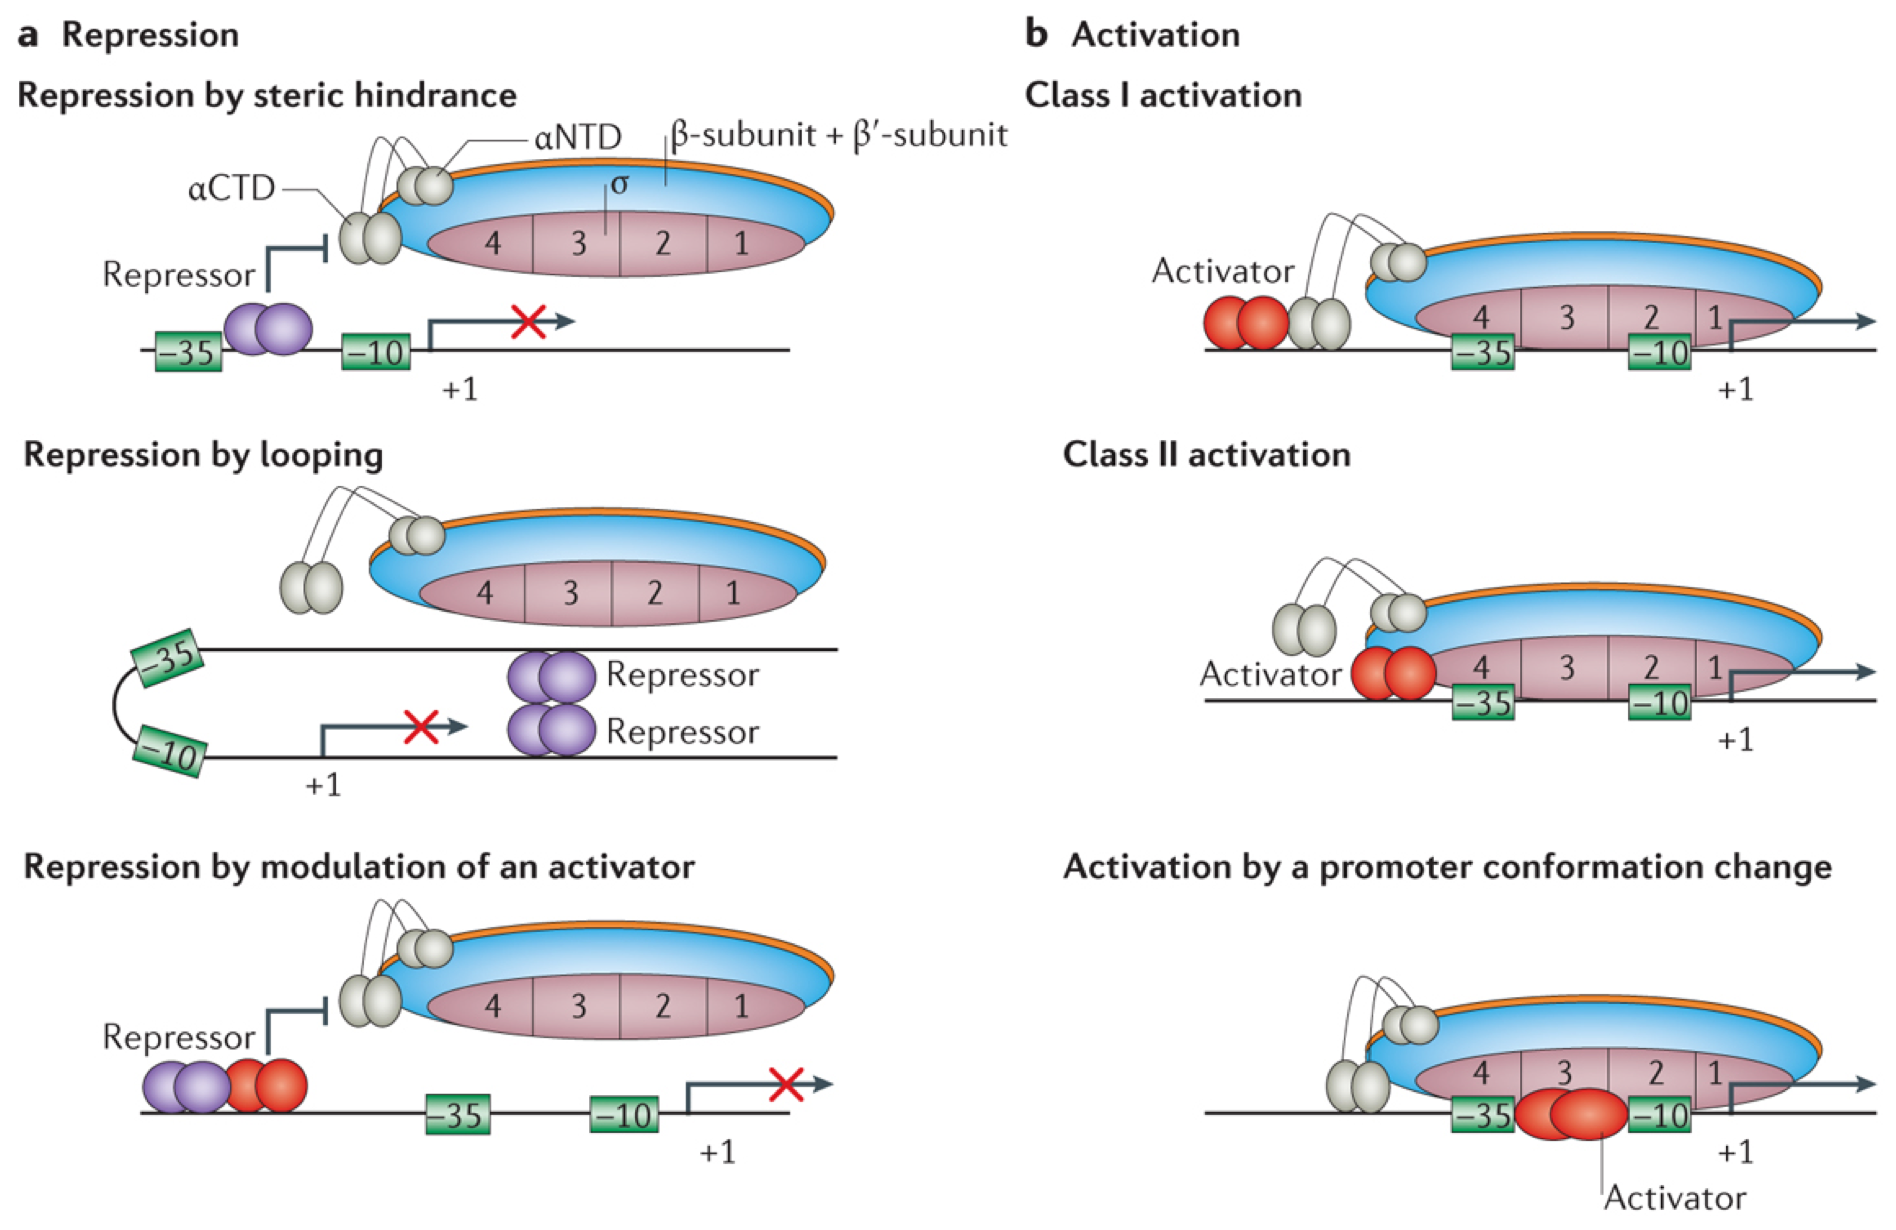
\includegraphics[scale=0.4]{text/Pictures/TxnInitRegulation.png}
	\caption{Regulation of transcription initiation by repressors and activators. (reproduced from \cite{browning2016local})}
	\label{txn}
\end{figure}

\textbf{Activation}, on the other hand, enables particular gene transcription or increases strength of RNA polymerase binding to the promoter.
Similar to the repression, some activators interact directly with RNA polymerase but other act indirectly as anti-repressors most often by releasing and preventing repressor binding to the operator \cite{frederix2011co}.
Besides affecting sequence specific repressors, some indirect activators affect also binding of NAPs, thus opening an access for RNA polymerase to the promoter sequence \cite{santana2001transcriptional}.
Direct activators mostly facilitate the very interaction of RNA polymerase and promoter.
Three mechanisms of direct activation are usually described: class I activation, class II activation and activation by conformational change.

Class I activators bind upstream of -35 element and interact with $\alpha$ subunit of RNA polymerase \cite{ushida1990helical} (Fig.~\ref{txn}\textcolor{red}{b}).
Operators of class II activators in turn overlap with -35 promoter element and the activators interact with given $\sigma$ factor of RNA polymerase \cite{igarashi1991functional} (Fig.~\ref{txn}\textcolor{red}{b}).
Moreover bound class II activator prevents binding of the RNA polymerase $\alpha$ subunit to the preferred position right upstream of -35 element.
Class I and class II activation thus can occur simultaneously on the same promoter when two different activators are required to trigger the transcription \cite{lloyd2002requirement}.

The last classical activation mechanism causes a conformational change of the sequence between -10 and -35 elements.
RNA polymerase binding to these promoters without activator is weakened or impaired due to inappropriate distance between -10 and -35 elements.
And this is also where the operators of such activators are located (Fig.~\ref{txn}\textcolor{red}{b}).
A bound activator then brings the elements into the optimal position for RNA polymerase recruitment \cite{heldwein2001crystal}.

All activation mechanisms mentioned above just enable RNA polymerase binding strong enough for an efficient transcription initiation.
Other kind of activation of transcription initiation is not even required for most RNA polymerase holoenzymes.
However, RNA polymerase containing $\sigma^{54}$ factor is unable to unwind promoter DNA to begin transcribe.
This is facilitated by enhancer binding proteins (EBPs) which interact with the $\sigma^{54}$ factor \cite{morett1989vivo, cannon2000dna}.
Nevertheless, EBPs bind upstream of the promoter elements, so to get in contact with the $\sigma^{54}$ factor a loop has to be produced.
Production of this loop is known to be mediated by nucleoid associated protein IHF which as well as other NAPs plays a role in DNA accessibility \cite{de1991upstream, sze2001vivo}.

\subsubsection{Regulation of mRNA elongation and transcription termination}
After a successful transcription initiation the elongation of mRNA follows until termination comes to place.
Even though the main transcription regulation occurs at the level of transcription initiation, elongation and termination can be also modulated, ranging from repression of elongation \cite{monsalve1996protein}, through elongation pausing and backtracking \cite{mustaev2017transcription} to transcription attenuation and anti-termination \cite{naville2009transcription}.

To the end of the section about transcription regulation it is good to point out the complexity of the whole process.
Even when both global and specific regulation of transcription initiation permit transcript production the gene expression is still regulated further downstream e.g. during mRNA elongation or translation.
Moreover one transcription factor can regulate multiple genes as well as being co-regulated by several factors including itself.
Regulation of gene expression thus exhibit a huge network of mutually controlled outputs based on the information acquired by a cell.

\subsection{Regulatory kinetics}
For better understanding of the whole transcription network regulation, it is important to look at the speed of different regulatory circuits as well.
This is usually characterised by a rise-time (or response time), i.e. time when the concentration of a gene product reaches its half maximal concentration after gene induction.

\subsubsection{Promoter strength and protein lifetime}
Naturally the more easily and often RNA polymerase binds effectively to a promoter the more of an appropriate protein is produced at the time.
The strength of the promoter is given by its nucleotide sequence and binding of transcription factors increases or decreases RNA polymerase affinity to it.
On the other side of this equilibrium is degradation of the product, as its stability in certain conditions determines its lifetime.
A functional protein is also diluted during cell division, which further reduces its amount per cell.

\subsubsection{Transcriptional network motifs}
As an additional fine tuning of transcriptional response speed the simple network motifs themselves can be considered (Fig.~\ref{motifs}).
It has been shown that a negatively autoregulated gene (Fig.~\ref{motifs}\textcolor{red}{a}) reaches equilibrium concentration much faster than if it is not autoregulated \cite{rosenfeld2002negative}.
In other words negative feedback loop shortens the product rise-time.
It also reduces the variability in product concentration maintaining it in optimal concentration limits \cite{becskei2000engineering}.
This enables the cell to use stronger promoters for proteins needed in a short time but at low concentration without overshoots and risks of protein toxicity.

Positive autoregulation (Fig.~\ref{motifs}\textcolor{red}{b}) exhibits right the opposite traits.
Slower and noisier initial response to gene activation is observed in case of positive feedback loops compared to no feedback systems \cite{maeda2006regulatory, sayut2007noise}.
Although it takes longer for the cell to reach certain level of desired protein, this motif allows to react to much lower concentrations of signal.
Moreover, both graded and hysteretic expression can be observed in positively autoregulated genes \cite{maeda2006regulatory}.
%%% IS THIS ENOUGH TO MENTION DIFFERENCE IN GRADED AND BINARY RESPONSE IN HERE OR DO YOU WANT ME TO EXPAND IT MORE IN e.g. A SEPARATE PARAGRAPH?

\begin{figure}[ht!]
  \centering
  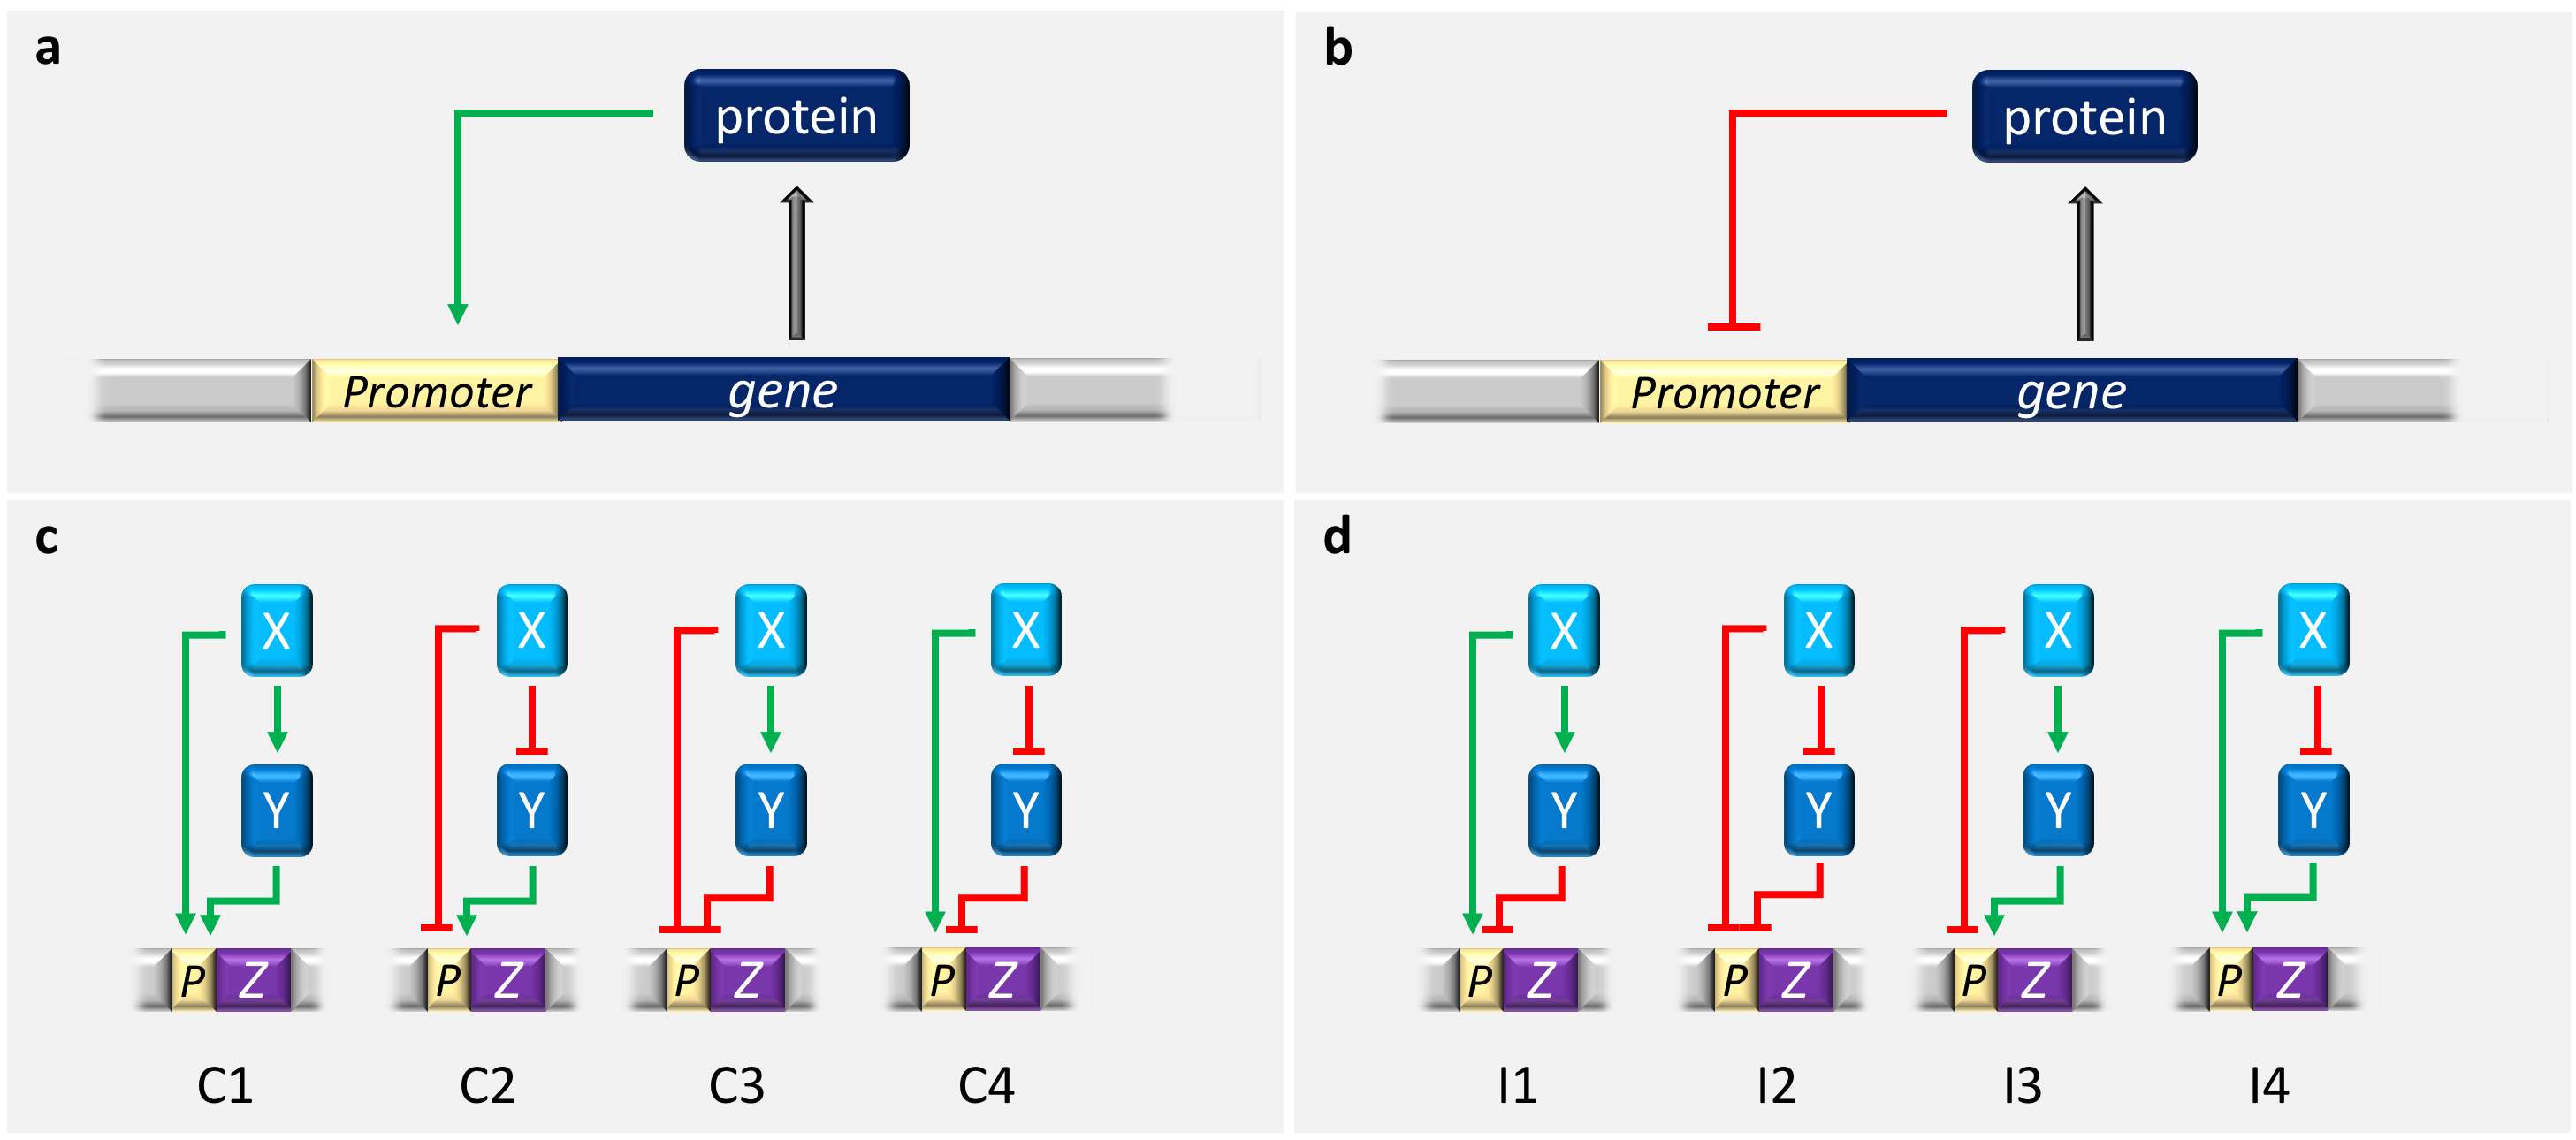
\includegraphics[scale=0.29]{text/Pictures/TxnMotifs.png}
	\caption{Schemes of transcriptional network motifs; \textbf{a} negative feedback loop - gene product represses its own transcription; \textbf{b} positive feedback loop - gene product induced transcription of its own gene; \textbf{c} coherent feed-forward loops; \textbf{d} incoherent feed-forward loops.}
	\label{motifs}
\end{figure}

Next common regulatory motifs in \tax{E. coli} are feed-forward loops (FFLs).
% the grammar in the next sentence is a bit off.
% there's a lot of abbreviations (e.g. FFL) and X factors piling up here. Can you change "X" to something mroe reader friendly? Not sure what / how...
By FFL is meant a regulatory circuit when a transcription factor X regulates other transcription factor Y and both (X and Y) regulate a gene or operon Z (Fig.~\ref{motifs}\textcolor{red}{c} and \textcolor{red}{d}).
There is further distinction between coherent and incoherent FFL.
When the regulation of Z by factor X has the same sign (positive or negative) as regulation of Z by X through Y we talk about coherent FFL (Fig.~\ref{motifs}\textcolor{red}{c}).
If the signs are opposite the FFL is considered incoherent \cite{shen2002network} (Fig.~\ref{motifs}\textcolor{red}{d}).
It has been predicted that coherent FFLs cause sign-sensitive delays in regulatory kinetics and incoherent FFLs should act as sign-sensitive accelelators and exhibit transient pulses of expression \cite{mangan2003structure}.
The most abundant schemes were later experimentally confirmed.
%%% IT'D BE GOOD TO HAVE PICTURE TO SUPPORT THE LAST SENTECE OF THE PARAGRAPH.

In coherent FFL type 1 (Fig.~\ref{motifs}\textcolor{red}{c},C1) factor X activates factor Y expression and both X and Y positively regulate transcription of Z \cite{mangan2003structure}.
There are two possible ways of induction of Z expression in this system.
First, both factors X and Y has to bind Z promoter to trigger transcription - AND-gate logic (AND-FFL).
Or only one of both is sufficient to activate Z gene - OR-gate logic (OR-FFL).
The AND-FFL was shown to delay full gene expression compared to non-FFL system \cite{mangan2003coherent}, while no delay was observed in the inverse (ON to OFF) transition.
To test OR-FFL a system where X and Y act in additive manner to activate Z was used and termed as SUM-FFL \cite{kalir2005coherent}.
This motif behaves right the opposite way than AND-FFL.
Transition from OFF to ON shows no delays.
But when factor X was deactivated the ON to OFF step was considerably delayed in comparison with strain with deleted gene for factor Y.
The former motif (AND-FFL) thus prevents Z expression when concentration of X fluctuates close to a threshold, while the latter circuit (SUM-FFL) enables continuous production of Z even if X concentration drops below a threshold for a while.

From incoherent FFL motifs the type 1 (Fig.~\ref{motifs}\textcolor{red}{d}, I1) is predominant in \tax{E. coli} transcriptional network.
Factor X here positively regulates both Y and Z, however factor Y acts as an inhibitor of Z gene.
The model predicted this incoherent FFL to speed up transcriptional responses, but weak pulse-generating power was expected \cite{mangan2003structure}.
Nevertheless this motif was used to create effective pulsers \cite{basu2004spatiotemporal}.
Later the acceleration trait was experimentally confirmed as well despite the fact that other motifs contribute to the used regulatory system \cite{mangan2006incoherent}.
This suggests that the motifs' fundamental functions are preserved even when combined with other motifs.
Overall this type of regulation similarly to negative feedback loop shortens the rise-time, but unlike the negative feedback doesn't avoid overshoots rather the opposite.
The overshoot is seen as a pulse of high gene Z expression which is subsequently inhibited by factor Y, but not necessarily back to the basal level.


\section{Epigenetics in bacteria}
Epigenetics is understood as a heritable change in gene expression without simultaneous changes in DNA primary sequence.
Some studies has shown that cells with the same genetic background might react differently or at a different rate to the same stimulus based on their and their ancestors recent experience \cite{mathis2017asymmetric, ronin2017long}.
Such ability is advantageous especially if the change in the conditions is predictable and repeats periodically.

\subsection{Mechanisms of bacterial memory}
Various epigenetic mechanisms such as histone modifications, genomic imprinting or RNA associated silencing are well studied in eukaryotes \cite{durso2014mechanisms}.
In bacterial domain DNA methylation by methyltransferases is mostly mentioned, although positive and double negative feedback loops play their role as well especially in terms of population bistability \cite{casadesus2006epigenetic, casadesus2013programmed, adhikari2016dna}.

% 2018.06.28
% Eventually, go into way more detail here, as this will end up as a full section on lac. But if you are leaving this as a brief intro to positive, negative, double negative, that's fine. You might also start with sensing/reaction and then move to epigenetics. This is a reasonable ref I think *An introduction to systems biology: design principles of biological circuits*, although you always have to be a little careful with Uri Alon's take on things, sometimes it's a bit too facile.
\subsubsection{Feedback loops}
System where a product is able to affect positively or negatively its own production is called a feedback loop.
The influence of the output on itself might be direct or indirect if multiple effectors are involved.
Feedback loops are quite common in bacterial gene regulation and can lead to epigenetic switches \cite{smits2006phenotypic, veening2008bistability}.
Positive feedback loop and double negative feedback loop are known to play a role in memory of prokaryotes so far and are characterized in detail below.

\textbf{Positive feedback loop} is the first described example of bacterial epigenetics.
It was shown already in 1957 that \tax{E. coli} sub-population primed by high concentration of lactose analogue TMG is able to maintain \tax{lac} operon fully induced even in low non-inducible TMG concentrations \cite{novick1957enzyme}.
While if the same bacteria are exposed to the low non-inducible TMG concentration without priming the \tax{lac} operon remains repressed by LacI.
The mechanism behind this resides in different levels of $\beta$-galactoside permease (LacY) in TMG induced and naive cells.
Induced population has high level of the permease present in membrane as \tax{lacY} gene expression is activated by high TMG concentrations.
This state is preserved in a sub-population of induced cells after transfer into low TMG concentration as the abundant permease is able to maintain intracellular TMG level high enough to avoid LacI repression.
Thus the high level of permease leads to high intracellular TMG concentration which in turn acts as permease transcription activator.
On the other side naive cells have very small amounts of LacY if any thus they are not able to obtain TMG from the solution to activate \tax{lac} operon expression \cite{smits2006phenotypic, casadesus2013programmed}.

\begin{figure}[h!]
  \centering
  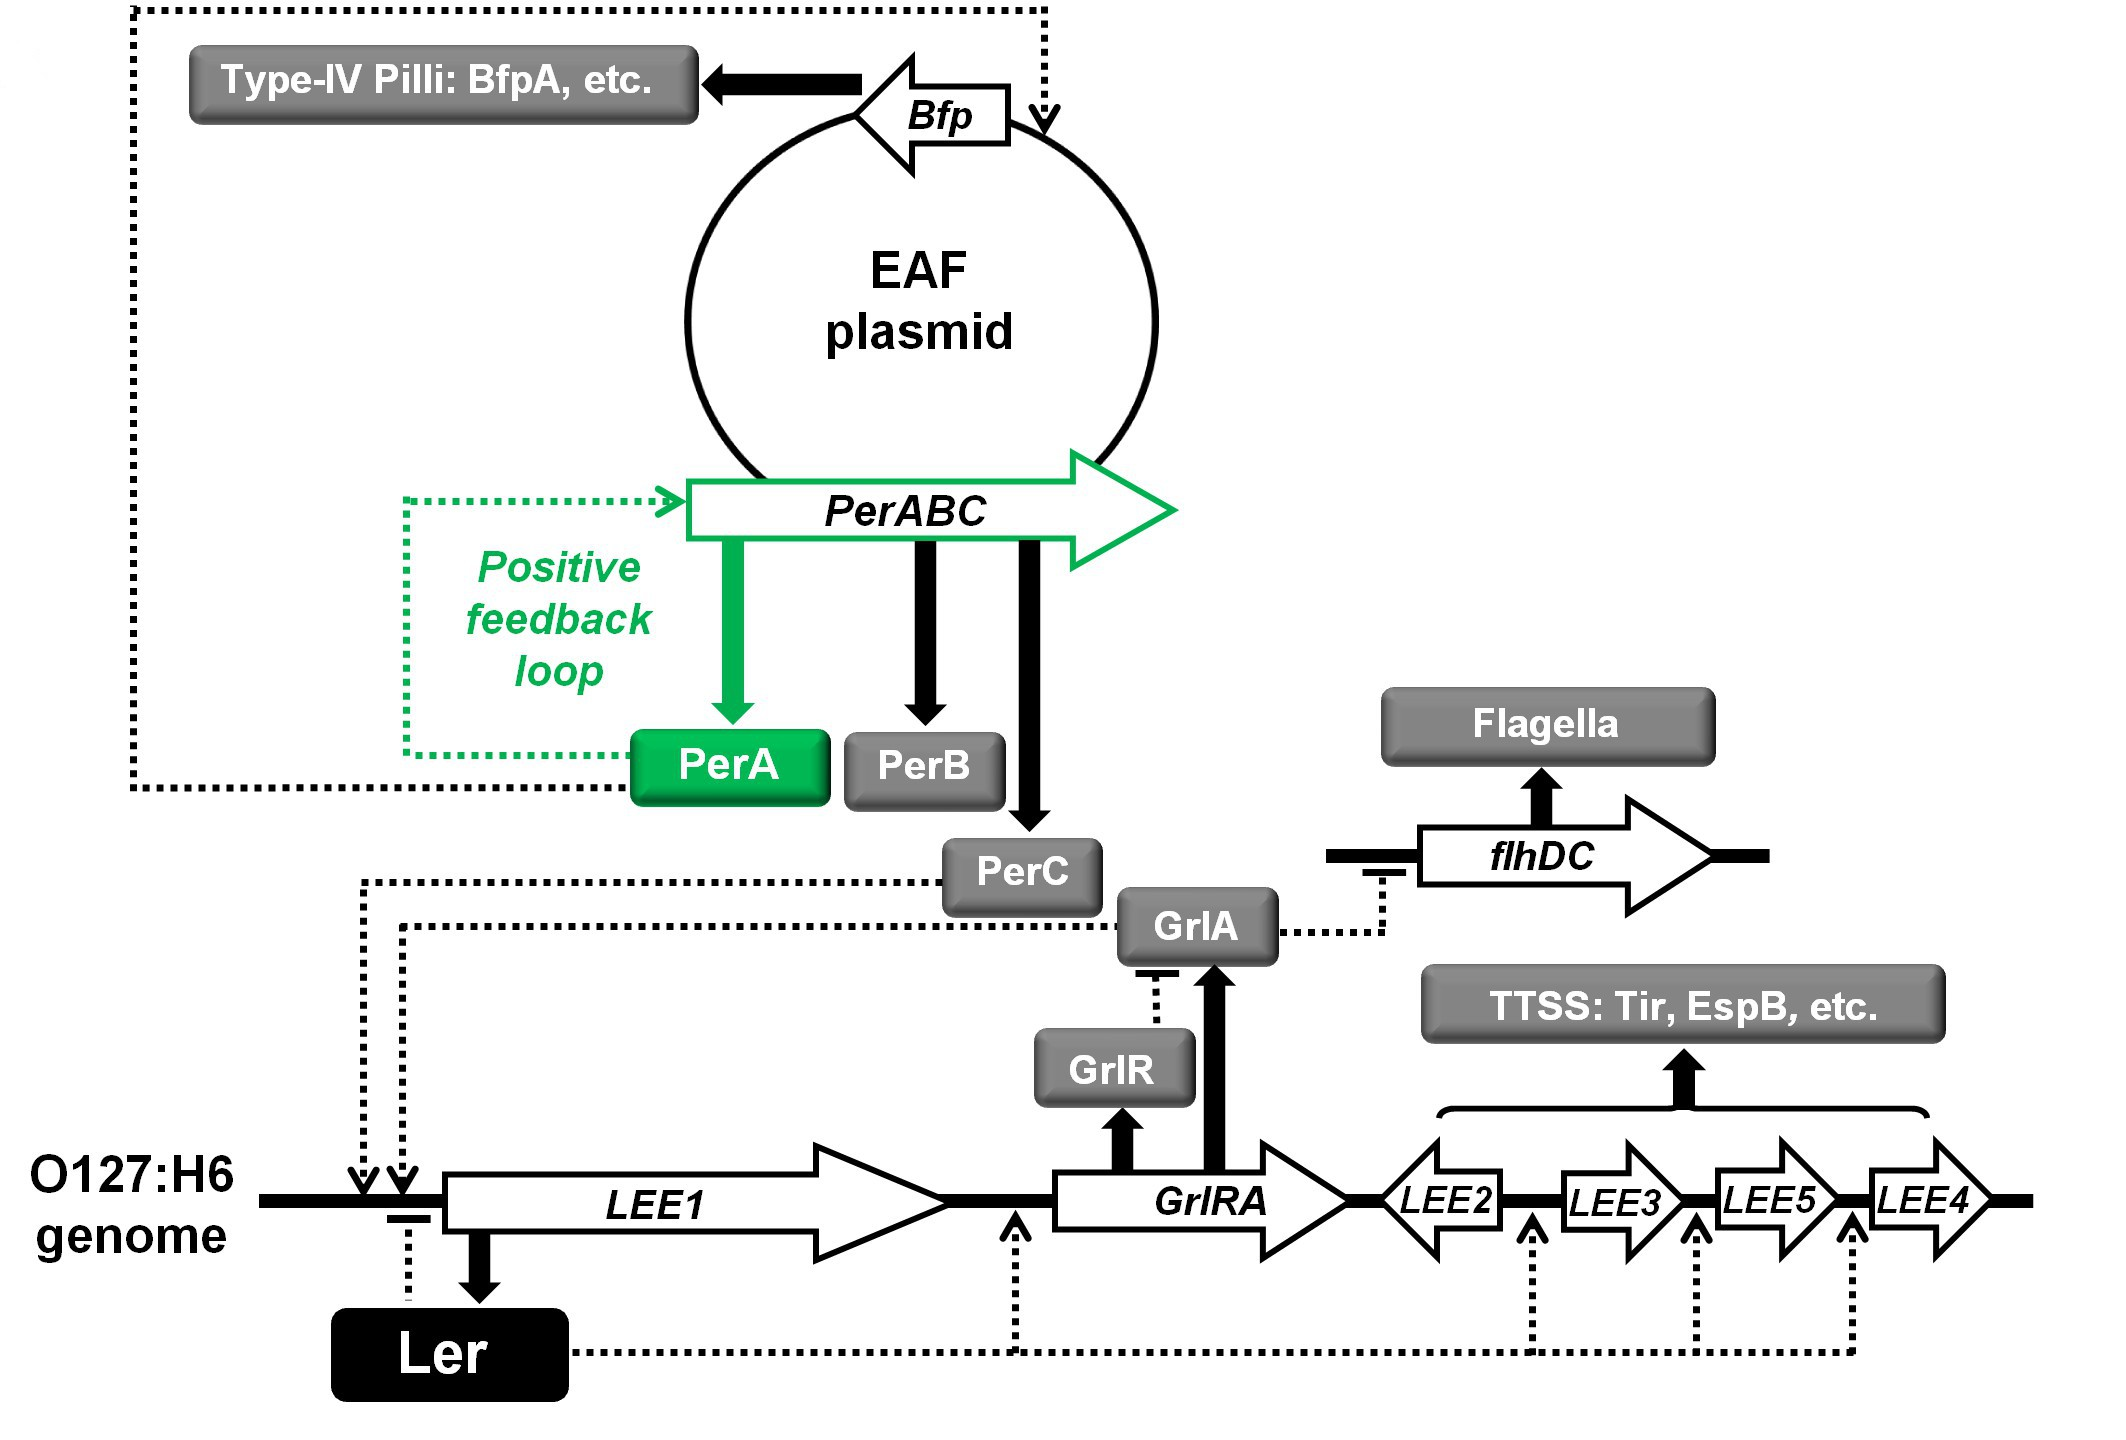
\includegraphics[scale=0.2]{text/Pictures/perOperonRegulation.jpg}
	\caption{Scheme of EPEC virulence regulation. PerA positivelly autoregulates \tax{perABC} operon and the triggers expression of type IV pili. PerC activates transcription of Ler which is the main regulator of T3SS secretion system machinery. (reproduced from \cite{ronin2017long})}
	\label{per}
\end{figure}

Another nice example of a long-term virulence epigenetic switch mediated by a positive feedback loop was published last year.
Enteropathogenic \tax{E. coli} (EPEC) coexists in two, non-virulent and hyper-virulent, sub-populations during growth \cite{ronin2017long}.
This bimodality was first observed  using ScanLag \cite{levin2014scanlag} as a difference in growth rates of the two groups resulting in BIG and SMALL colony morphotypes, for early and late appearing colonies, respectively.
At transcription level it is a change in \tax{per} operon expression (located on EAF plasmid) and \tax{per} regulated genes.
EPEC cultivation in virulence-activating conditions gives rise to \tax{per}-ON hyper-virulent aggregative sub-population (SMALL phenotype) reaching nearly 100\% \cite{ronin2017long}.
Interestingly this high ratio of \tax{per}-ON vs \tax{per}-OFF cells remains for many generations even after transferring the culture back into non-activating conditions, although naive EPEC culture contains only a minority of \tax{per}-ON cells.
Transition back from \tax{per}-ON to \tax{per}-OFF phase is achieved when cells are grown up to stationary phase.
The long-term stability of \tax{per}-ON state relies on a positive feedback of PerA which acts as an activator of its own gene beside \tax{perB} and \tax{perC} in the \tax{per} operon (Fig.~\ref{per}) \cite{ibarra2003identification, ronin2017long}.
%%% More examples of positive feedback to add???

As an illustration of \textbf{double negative feedback loop} in epigenetic regulation a switch between lytic and lysogenic cycle of \tax{E. coli} phage $\lambda$ is often described \cite{smits2006phenotypic, casadesus2013programmed}.
After inserting its DNA the virus cycle might undergo two different ways - i.e. either replicate producing a lot of new phages and heading for bacterial lysis or integrate its own DNA into the bacterial chromosome and persist there within a lysogeny.
The fate of the phage lies in two repressors, CI and Cro, each repressing transcription of the other \cite{eisen1970regulation, neubauer1970immunity}.
Besides CI inhibits phage propagation genes and activates its own transcription.
However, both CI and Cro are produced since the beginning of the infection.
If the level of CI reaches a certain threshold and outcompetes Cro, whose activity is suppressed, the phage enters a lysogenic cycle staying dormant in the cell thanks to CI-\tax{cI} positive feedback loop.
Otherwise Cro levels rise further inhibiting CI production and establishing phage proliferation with subsequent cell lysis \cite{svenningsen2005role}.
It should be noted that although it is not predictable whether the phage enters lytic or lysogenic cycle, the ratio of lysed/lysogenized cells depends on bacterial physiologic situation and other environmental factors as well.
Interestingly, Toman et al. used the CI-Cro system for epigenetic reuglation of \tax{gal} operon in \tax{E. coli} \cite{toman1985system}.
%%% it's not epigenetics in E. coli, but in the phage lambda! (except for the engineered system by Toman et al.)

%%%As the CI-Cro regulation is a phage system, the first evidence of bacterial epigenetics driven by a double negative feedback loop was published just 3 years ago.

%%% detection of double negative feedback loop originating in bacteria?
%%% double negative feedback detected in "A Novel Feedback Loop That Controls Bimodal Expression of Genetic Competence" which talks about cell competence
%%% there is no direct evidence for epigenetics playing role in it, however paper "Agent-based modeling of competence phenotype switching in Bacillus subtilis" suggests it might be so according to their model
%%% especially when in similar case - bacillus sporulation is it proven in: "Bet-hedging and epigenetic inheritance in bacterial cell development"

\subsubsection{DNA methylation by orphan methyltransferases}
% in my opinion you can shrink this section a bit.
% one thing to note is that you have gone back and forth between very general topics (the toplogy of regulation networks), to more specific mechanisms (regulating txn via TFs), to very specific mechanisms (dam / dcm). Don't dive too deep. Deep dives into very particular cellular mechanisms can be for later (e.g. if you end up doing a lot fo work on one type of mechanism).

Orphan methyltransferases (MTs) were initially studied within restriction-modification system as a bacterial defence against phages, although Dam's ability to alter some gene expression was already described in mid-80s \cite{sternberg1985evidence, bickle1993biology}.
As orphan MTs lack their cognate restriction endonucleases their role in bacterial cells is not as a primitive immune system, but among others can act as a transcription regulators.
I describe the epigenetic mechanisms of Dam in detail below as the MT whose relationship to cell memory is most understood.
Some authors consider the change in expression of certain genes in \tax{Caulobacter crescentus} which is associated with an orphan MT called CcrM to be epigenetic as well \cite{casadesus2006epigenetic, adhikari2016dna}.
However I do not include it here as these transcriptional changes are not heritable and occur only during a part of a cell cycle.
Other \tax{E. coli} orhan MTs are mentioned briefly as well although none of them is known to play a role in epigenetics so far.

\textbf{Dam}, one of two first orphan MTs described in \tax{E. coli}, methylates adenine in 5'-GATC-3' sequences to N$^6$-methyladenine (6mA) \cite{marinus1973isolation}.
Its homologs were found in some bacteriophages as well as in other \tax{Gammaproteobacteria}, however many of bacterial DNA adenine methylases are associated with restriction endonucleases \cite{low2001roles, casadesus2006epigenetic, bochow2012bacteriophage}.
On the other hand strains having an orphan DNA adenine methylase can be characterized by presence of SeqA and MutH, overrepresentation of GATC sites in \tax{oriC}, genes close to it and in the \tax{dnaA} promoter \cite{sobetzko2016distamo}.
For most of the DNA both strands of chromosome are fully methylated throughout the cell cycle if Dam is present.
Of course, one of the exceptions is a short time hemimethylation of a leading strand and Okazaki fragments right after their synthesis during replication.
Both strands lack GATC methylation in \tax{dam} mutants, moreover higher mutation rate, uncoordinated replication initiation or loss of virulence were observed as well.
Interestingly for some species e.g. \tax{Vibrio cholerae} the presence of an orphan DNA adenine methylase is vital, whereas it is non-essential for other, such as \tax{E. coli} \cite{casadesus2006epigenetic, casadesus2013programmed, adhikari2016dna}.

As implied above several GATC sites escape Dam methylation.
This happens if another regulatory protein recognises a specific DNA biding site which overlaps GATC sequence and thus competes with Dam for it \cite{correnti2002dam}.
Such mechanism leading to epigenetic switch is well characterized in synthesis of \tax{pap} pili in uropathogenic \tax{E. coli} (UPEC) \cite{peterson2008competitive}.
The regulatory sequence of the \tax{pap} operon contains two sets of Lrp binding sites 1-3 and 4-6.
In both of them GATC sequence is present, GATC$^{prox}$ within site 2 and GATC$^{dist}$ within site 5 (Fig.~\ref{pap}) \cite{blyn1990regulation}.

% This is good. Maybe label the lrp sites as you refer to them in the text?
\begin{figure}[h!]
  \centering
  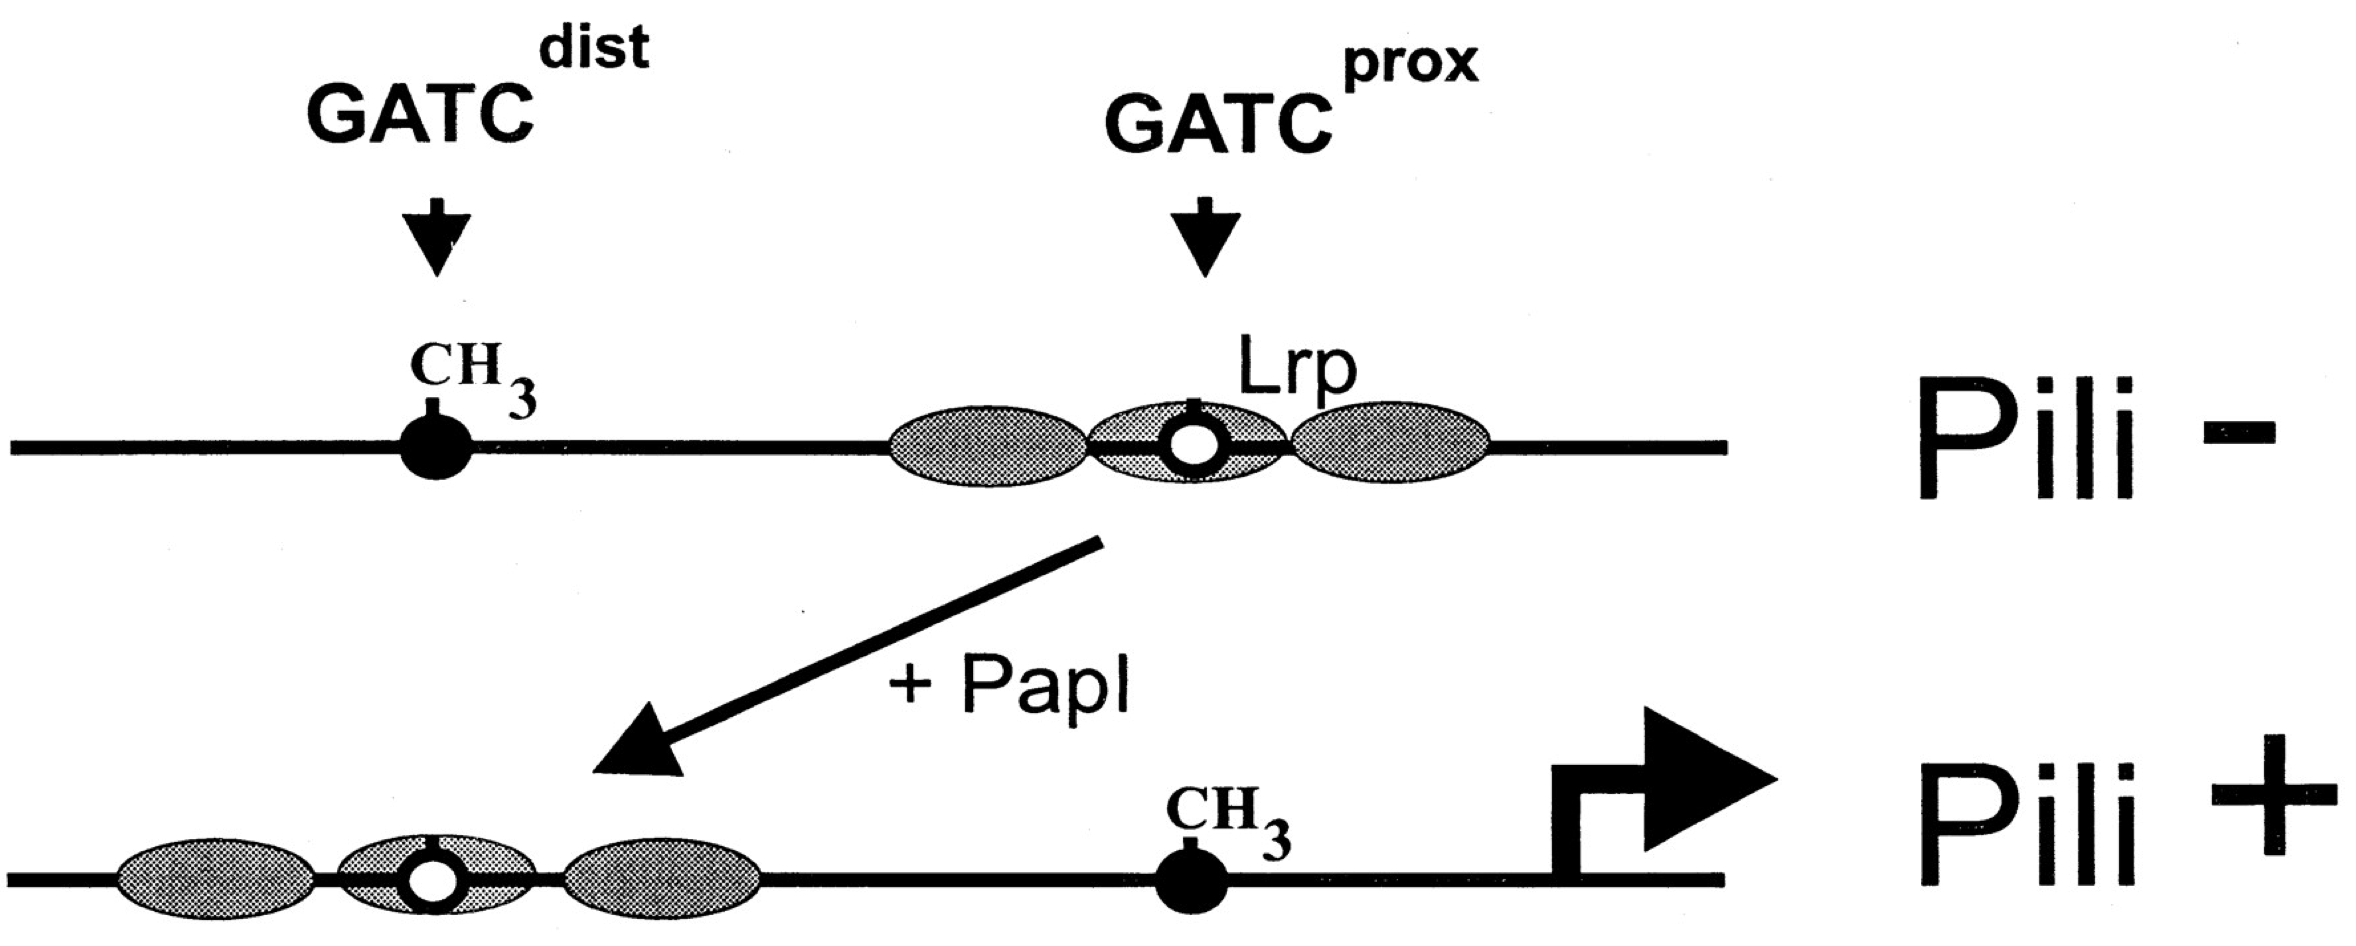
\includegraphics[scale=0.3]{text/Pictures/papPili.png}
	\caption{Scheme of the \tax{pap} phase OFF to ON switch. (reproduced from \cite{low2001roles})}
	\label{pap}
\end{figure}
During the OFF phase \tax{pap} pili are not produced because Lrp occupies GATC$^{prox}$ site which remains nonmethylated on both strands while GATC$^{dist}$ is fully methylated.
Lrp in this position prevents binding not only by Dam but by $\sigma^{70}$ RNA polymerase as well inhibiting expression of \tax{papBA} gene \cite{weyand2000regulation}.
For switch to ON phase an initial Lrp dissociation from sites 1-3 is necessary.
This likely happens during replication when an opportunity for Lrp to bind the hemimethylated GATC$^{dist}$ site instead of GATC$^{prox}$ raises.
The probability of this switch depends on the level of regulatory protein PapI in the cell as complex PapI/Lrp has lower affinity to site 2 but binds more likely to hemimethylated sites 4-6 than to fully methylated DNA \cite{hernday2003mechanism}.
Besides Lrp release from GATC$^{prox}$ site enables access of Dam to it so it can become methylated which further reduces Lrp affinity to 1-3 sites.
Even though RNA polymerase's access to \tax{papBA} promoter is not blocked any more the expression itself requires cAMP-CAP \cite{weyand2001essential}.
When PapB is beeing produced it acts as a \tax{papI} gene transcription activator leading to a feedback loop which stabilizes the cells in ON phase \cite{forsman1989autoregulation}.
However the described transition from OFF to ON phase occurs with 100-fold lower frequency than vice versa \cite{blyn1990regulation}.
The process of this opposite transition i.e. from ON to OFF phase involves transfer of Lrp from GATC$^{dist}$ to GATC$^{prox}$ during replication but the exact mechanism is not fully understood yet \cite{adhikari2016dna}.

Another well known orphan MT in \tax{E. coli} is \textbf{Dcm} which methylates second cytosine in 5'-CC(A/T)GG-3' motif to 5-methylcytosine (5mC) \cite{marinus1973isolation}.
Even though neither this one is necessary for \tax{E. coli} survival and some strains were found lacking \tax{dcm} gene, link between certain genes expression and presence of this MT was described.
Dcm seems to slow down expression of ribosomal genes \tax{rplC} and \tax{rpsJ} and inhibit transcription of \tax{sugE} gene connected with higher antimicrobial resistance \cite{militello2012conservation, militello2014cytosine}.
Both is happening predominantly during early stationary phase.
Next study shows increased expression of stress response sigma factor RpoS in \tax{dcm} mutant \cite{kahramanoglou2012genomics}.
Recently additional 63 genes were discovered to be affected if Dcm activity is inhibited \cite{militello20165}.
Most of these genes are up-regulater during early stationary phase if methylation by Dcm is silenced.

Lastly \textbf{YhdJ} is an orphan MT methylating 3' adenine of 5'-ATGCAT-3' sequence to 6mA when overexpressed.
Deleting \tax{yhdJ} gene produces neither loss of viability of \tax{E. coli} nor changes in its phenotype.
In addition, the expression of the gene is very low under usual laboratory conditions and nothing is known about transcription regulation of the gene \cite{broadbent2007yhdj}.

\subsubsection{Protein aggregation}
At the end of previous month a new mechanism of bacterial memory was described \cite{govers2018protein}.
Protein aggregates (PAs) which are usually formed in response to a proteotoxic stress (e.g. sub-lethal heat-shock) were found to protect cells which bear them against new proteotoxic stresses.
Those PAs are asymmetrically divided between daughter cells and gradually disaggregated.
However, the disaggregation of PAs is very slow.
This thus provides a long-time memory in PA-bearing cells of such past events.
The authors show that cells which inherit protein aggregates are more likely to survive sub-lethal heat-shock or streptomycin exposure.
They also resume growth much earlier than genetically identical cells without PA.
%%% DO YOU WANT ME TO WRITE MORE ABOUT THIS?

\subsection{Predictive cell behaviour}
An ability to predict an upcoming change in the environment is beneficial for any organism.
No matter whether the change means a presence of antibiotic or just shift in carbon source availability.
If a bacterium is able to predict such event it has a fitness advantage over those who don't expect this to happen in that community.

Circadian rhythms in photoautotrophic Cyanobacteria can be considered as one example of predictive behaviour in bacterial world.
It consists of alternation between photosynthetic activity during day and nitrogen fixation at night.
This periodicity persists in complete darkness or light for days.
It can also be reset by light or dark pulses in a way that two genetically identical populations act in the opposite way (oxygen production or nitrogen fixation) in constant dark or light conditions at the same time \cite{kondo1993circadian}.
Similar oscillatory rhythm was described in a bacterium other than Cyanobacterium as well.
\tax{Rhodobacter sphaeroides} was observed to keep changing gene expression in circadian (aerobic conditions) or ultradian (anaerobic conditions) rythms \cite{min2005rhythmic}.
Recent study investigating connection between day-and-night cycle and overall gene expression of microbial mat suggest that daily rhythmicity might not be uncommon outside Cyanobacteria \cite{hornlein2018daily}.
They state that 50\% of the rhythmic genes was derived from phylum \tax{Proteobacteria}.

Next predictive behaviour with no connection to day-and-night regime was observed in \tax{E. coli}.
Naturally it faces recurrent transitions between mammalian gastrointestinal tract (GIT) - higher temperature, lower oxygen - and outside environment - lower temperature, higher oxygen.
Consistent with predictive behaviour \tax{E. coli} strongly represses genes responsible for aerobic metabolism to temperature increase (without change in oxygen levels) in laboratory conditions \cite{tagkopoulos2008predictive}.
While if the temperature drops correlation in up-regulation of aerobic metabolism genes occurs.
They also evolved this strain in conditions where an increase in temperature was followed by oxygen saturation and temperature decrease by anaerobic conditions.
The two responses were successfully decoupled after 1000 generations suggesting that anticipatory regulation can be evolved for and against.

A year later, prediction of maltose environment to lactose exposure in \tax{E. coli} was described \cite{mitchell2009adaptive}.
Evolution under high lactose concentrations without maltose resulted in loss in prediction of maltose exposure and evolved lines exhibit a big fitness disadvantage compared to ancestor upon lactose-maltose transition.
The same authors investigated anticipation of oxidative stress by yeast which occurs in its natural habitat upon transition from fermentation to respiration.
\tax{Saccharomyces cerevisiae} uses heat-shock, ethanol and low pH as cues to prepare for its coming without actually experiencing it at the time \cite{mitchell2009adaptive}.


\section{Natural selection on responses and memory}
The current knowledge about gene expression in prokaryotes shows that transcription is a fairly regulated process.
But how this regulation evolved under selection in natural conditions is not fully understood.
Hypothesis about selection acting on transcriptional sensitivity, noise and possible memory exist.
%%% FIND REFERENCES FOR THAT!!!
Some supporting evidence and experiments exist, yet a lot remains to unravel still.

\subsection{Selection on sensitivity}
It was mentioned above that cells possess mechanisms to modulate time-dependent sensitivity of gene expression to a signal (e.g. FFLs).
Some of them are overrepresented in living organisms over others compared to randomized networks \cite{shen2002network, mangan2003structure}.
Bacteria are thus under natural selection towards accurate timing of their responses.
But is concentration-dependent sensitivity to a signal under selective pressure as well?
Common sense says there should be selection towards the concentration of a signal that is informative in the particular environment.
To the best of our knowledge no research investigated this so far.
%%% OR SHOULD I SAY "MY" KNOWLEDGE?
A possible way how to look into whether selection acts to reach certain level of sensitivity of promoters to a signal level is through experimental evolution.
Sensitivity of promoter variants from natural isolates could be then compared to those of lines evolved under low to high levels of an appropriate signal.
Looking simply at the distribution of concentration sensitivity of naturally occurring promoters could also provide useful information in this matter.

\subsection{Selection on noise}
Prior works have clearly shown that expression noise is evolvable \cite{richard2014does}.
Generally essential, constitutional genes and genes with high effect on overall expression (i.e. some transcription factors) tend to have low transcriptional noise \cite{silander2012genome, metzger2015selection}.
In constrast another interesting study describes higher noise in promoters from natural isolates of \tax{E. coli} compared to those of experimentally evolved lines just for their mean expression \cite{wolf2015expression}.
These results suggest that for different genes and/or at different niches there is a different optimum of transcriptional noise.
Indeed, a very recent study of the effect of expression noise on fitness of \tax{Saccharomyces cerevisiae} reveals that high noise is beneficial when expression level is far from optimum and vice versa \cite{duveau2018fitness}.
They also indicate that after introduction of an organism into a new environment selection might act towards high noise in expression of some genes before an appropriate expression plasticity evolves.
However, note that mutations in promoter regions usually change both expression level and noise at the same time \cite{metzger2015selection}.
Some work in this area on other model organisms such as \tax{Drosophila melanogaster} \cite{schor2017promoter} and mouse \cite{barroso2017evolution} has been done as well.
But it still remains to validate that it is actually selected for certain levels of noise in natural environment by looking into noise variations of individual genes among distinct microbial isolates.

\subsection{Selection on memory}
As mentioned above some bacteria can react faster to a signal if they were exposed to the same singal in past \cite{novick1957enzyme}.
The development of microfluidics devices has enabled to study microbial adaptive memory at single cell level.
For example, sister and cousin cells have correlated lag times upon glucose-lactose media switch \cite{boulineau2013single, kaiser2018monitoring}.
LacY production in \tax{E. coli} continues after a short lactose pulse although the lactose is no longer present \cite{lambert2014memory} and \tax{E. coli} also keeps producing more LacZ even after reaching maximal growth rate and thus overshooting its actual need \cite{kaiser2018monitoring}.
Similar behaviour was observed e.g in yeast galactose system \cite{zacharioudakis2007yeast, razinkov2013measuring}.
But a question still remains: are these observed traits really what is actively selected for in natural fluctuating environment in order to remember past events for several generations?

Some bacteria are also able to predict upcoming event based on othervise unrelated signal \cite{kondo1993circadian, min2005rhythmic, tagkopoulos2008predictive, mitchell2009adaptive}.
An attempt of evolution of classical Pavlovian reflex to originally neutral signal in microorganisms was published last year \cite{lopez2017adaptive}.
As the neutral signal caffeine was added to media which yeast \tax{S. cerevisiae} was expected to associate with upcoming 5-fluoroorotic acid presence (metabolised into a toxic substance).
This predictive-like response appeared just within few hundred generations, but was not stable over time.
Thus, little is still known how microorganisms evolve such reflex to neutral cues.
A mathematical model suggests this to occur if benefits of such prediction exceed its costs in other environments \cite{mitchell2011mathematical}, but no experimental evidence is available so far.
Nevertheless the reported decoupling of reaction to a signal in the absence of expected outcome is an indication of selection acting on predictive behaviour \cite{tagkopoulos2008predictive, mitchell2009adaptive}.

Basically all work in this area has been done on single strains.
But the questions about how natural selection acts on transcriptional responses and memory in bacteria cannot be fully addressed without exploring natural variability in individual promoters among various isolates of the same genus.
Because without the knowledge of the natural phenotypic and genotypic variation in responses and memory we can just guess how selection forces shape these traits in nature, at what extent or whether they really do so.
And this is something no one have looked into in detail as yet.


\section{Natural variation in responses and memory}
Although the presence of \tax{E. coli} in water is still widely used as an indicator of fecal contamination, recent studies show that some \tax{E. coli} isolates are able to  reproduce in outside environment \cite{byappanahalli2004indigenous, somorin2016general}.
Moreover, strains inhabiting soil for a long time were found to be distinctive from those isolated from animals \cite{walk2009cryptic, walk2015cryptic}.
This raises the questions how these bacteria survive outside their hosts.
The ability of \tax{E. coli} to adapt to such different environments as animal gut and soil or water are, might also help us understand the evolution of promoters to fluctuating environments and bacterial memory.

When looking at adaptation of a species to various conditions, one should consider not only genotypic, but pheontypic variation as well.
It is now well known and generally accepted that even cells with the same genotype do not necessarily exhibit the same phenotype in identical conditions \cite{ronin2017long, govers2018protein}.
On the other hand various genetic backgrounds might still have very similar phenotype in some cases if evolution in environment with strong selection occurs.
In other words various strains might come to the same phenotype by different genotypic solutions.

\cleardoublepage

